\documentclass{beamer}

\usepackage{Haust2017glærur}

\title{Stærðfræðimynstur í tölvunarfræði}
\subtitle{Vika 4, fyrri fyrirlestur}

\begin{document}

\begin{frame}
\titlepage
\end{frame}

\section{Inngangur}

\begin{frame}{Í síðasta tíma}
\begin{itemize}
 \item Skilgreiningar reiknirita
 \item Lýsing og eiginleikar reiknirita
 \item Leitarreiknirit
 \item Röðunarreiknirit
 \item Gráðug reiknirit
\end{itemize}
\end{frame}


\section{Stöðvunarvandamálið}

\begin{frame}{Stöðvunarvandamálið}
\begin{itemize}
 \item Áður hefur verið haldið fram að óákvarðanleg föll séu til
 \item Sýnum nú að til sé vandamál sem ekkert forrit getur leyst
 \item Dæmi um slíkt vandamál er stöðvunarvandamálið (e. \emph{the halting problem})
 \begin{itemize}
  \item Forrit sem leysir stöðvunarvandamálið myndi geta tekið inn annars vegar forrit og hins vegar inntak í forritið og svarað hvort að forritið muni ná að ljúka keyrslu eða ekki 
 \end{itemize}
 \item Alan Turing sýndi að ekki er til forrit sem leysir stöðvunarvandamálið árið 1936
\end{itemize}
\end{frame}

\begin{frame}{Aths. um stöðvunarvandamálið}
    \begin{itemize}
    \item Athugum: Það dugar ekki einfaldlega að keyra forritið $P$ með inntakinu $I$ til að ákvarða vandamálið
    \begin{itemize}
    \item Ef $P$ klárar vitum við vissulega svarið\ldots
    \item \ldots en meðan það er enn að keyra vitum við ekki hvort það mun klára eftir eina sekúndu, eftir milljarð ára eða aldrei
    \end{itemize}
    \item Gerum kröfu um að forritið sé rétt, endanlegt og almennt
    \end{itemize}
\end{frame}

\begin{frame}{Sönnun með mótsögn}
\begin{itemize}
 \item Gerum ráð fyrir að við séum með forrit $H$ sem leysir stöðvunarvandamálið fyrir forrit $P$ og inntak $I$
 \begin{itemize}
  \item $H$ skilar strengnum ``stoppar'' ef $P$ stoppar gefið $I$ sem inntak, annars ``keyrir endalaust'' \pause
 \end{itemize}
 \item Athugum að forrit er safn tákna, svo forrit er strengur, streng má nota sem inntak
 \item Leysi $H$ stöðvunarvandamálið á það því að geta svarað því hvort $P$ stoppar þegar $P$ sjálft er notað sem inntak
\end{itemize}
\end{frame}

\begin{frame}{Sönnun með mótsögn}
\begin{itemize}
 \item Búum nú til forrit $K(P)$ sem notar $H(P, P)$
 \begin{itemize}
  \item Skili $H(P, P)$ strengnum ``keyrir endalaust'' stoppar $K(P)$ 
  \item Skili $H(P, P)$ strengnum ``stoppar'' fer $K(P)$ í endalausa lykkju
  \item $K(P)$ gerir sem sagt það gagnstæða við $H(P, P)$
 \end{itemize}
\end{itemize}
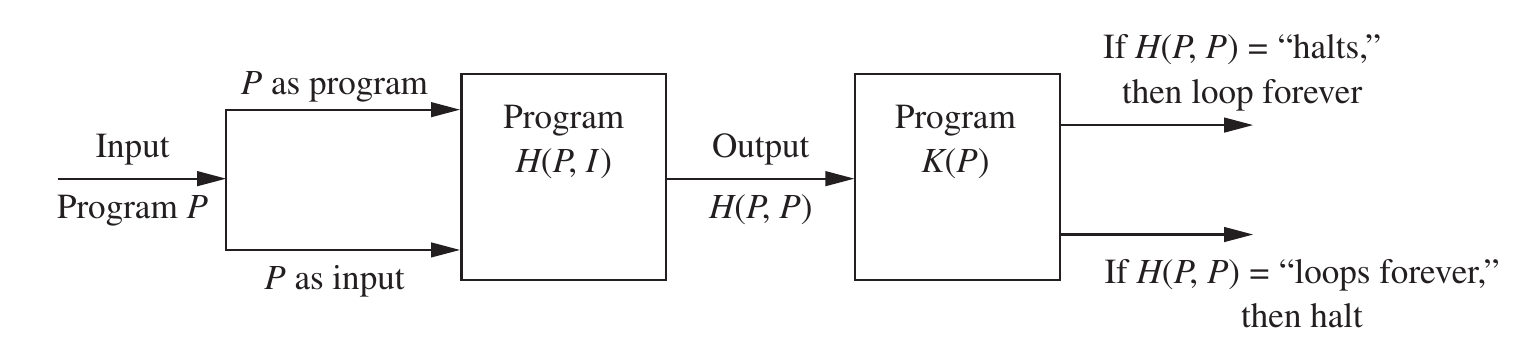
\includegraphics[width=\textwidth]{haltingproblem}

\pause
En hvað gerist ef við köllum á $K(K)$?
\end{frame}

\begin{frame}{Sönnun með mótsögn}
\begin{itemize}
 \item Ef $H(K, K)$ segir að $K(K)$ ljúki keyrslu, þá lýkur $K(K)$ ekki keyrslu
 \item Ef $H(K, K)$ segir að $K(K)$ ljúki ekki keyrslu, þá lýkur $K(K)$ keyrslu
 \item Mótsögn!
 \begin{itemize}
  \item Ekki er til $H$ sem leysir stöðvunarvandamálið fyrir öll forrit
 \end{itemize}
\end{itemize}
\end{frame}

\begin{frame}{Af hverju?}
    \begin{itemize}
        \item Gagnlegt er að vita af óleysanlegum vandamálum
        \item Til að sýna að vandamál sé óleysanlegt dugar að sýna að lausn á því myndi duga til að leysa stöðvunarvandamálið
    \end{itemize}
\end{frame}

\section{Stóra-O ritháttur}

\begin{frame}{Vöxtur falla}
\begin{itemize}
 \item Í stærðfræði dugar oft ágætlega að ákvarða hvort reiknirit leysi vandamál rétt á endanlegum tíma eða ekki
 \item Í tölvunarfræði þurfum við oftast líka að hugsa um hversu hratt er hægt að leysa þau
 \begin{itemize}
  \item Forrit sem leysir vandamál á einum milljarði ára er endanlegt og getur verið rétt, en er ekki sérlega gagnlegt
 \end{itemize}
 \item Innleiðum rithátt til að lýsa vexti falla
\end{itemize}
\end{frame}

\begin{frame}{Saga}
Rithátturinn sem oftast er notaður er kallaður stóra-O rithátturinn (e. \emph{big O notation}).

Rithátturinn var fyrst notaður af þýska stærðfræðingnum Paul Bachmann. Donald Knuth gerði ritháttinn vinsælan meðal tölvunarfræðinga.
\end{frame}

\begin{frame}{Stóra-O ritháttur}
\begin{tcolorbox}[title=Stóra O ritháttur]
Látum $f$ og $g$ vera föll frá $Z$ eða $R$ til $R$. Við segjum að $f(x)$ sé $O(g(x))$ ef til eru jákvæðir fastar $C$ og $k$ svo að

\[
 |f(x)| \leq C \cdot |g(x)|
\]

þegar $x > k$.
\end{tcolorbox}
Þetta þýðir að þegar $f(x)$ er $O(g(x))$ vex það hægar en eitthvað margfeldi af $g(x)$ þegar $x$ er ``nógu stórt''.
\end{frame}

\begin{frame}{Notkun ritháttarins}
\begin{itemize}
 \item Oftast er talað um að $f(x)$ ``sé'' $O(g(x))$ til að lýsa sambandinu
 \item Ekki alls kostar nákvæmt, þar sem $O(g(x))$ er mengi falla
 \begin{itemize}
  \item Gott væri að skrifa $f(x) \in O(g(x))$
 \end{itemize}
 \item Stundum er skrifað $f(x) = O(g(x))$
 \begin{itemize}
  \item Þetta er óheppilegur ritháttur!
 \end{itemize}
\end{itemize}
\end{frame}

\begin{frame}{Vitnin}
\begin{itemize}
 \item Fastarnir $C$ og $k$ mynda vitni (e. \emph{witness}) fyrir samband $f(x)$ og $O(g(x))$
 \item Nóg er að finna eitt vitni (hér eitt par fasta)
 \begin{itemize}
  \item Athugum að þegar við höfum fundið eitt vitni $C, k$ getum við alltaf fundið nýtt vitni $C', k'$, þar sem $C < C'$ og $k < k'$
  \item Þetta gildir því að $|f(x)| \leq C|g(x)| \leq C'|g(x)|$ þegar $x > k' > k$
 \end{itemize}
\end{itemize}
\end{frame}

\begin{frame}{Notkun}
Lauslegt dæmi: Er $x^2 + 2x + 1$ $O(x^2)$? \pause

Giskum á $k = 1$, svo $x > 1$. Þá vitum við líka að $x^2 > 1$ og $x^2 > x$. Þá setjum við upp:

\[
 0 \leq x^2 + 2x + 1 \leq x^2 + 2x^2 + x^2 = 4x^2
\]

Svo við getum notað $k = 1$ og $C = 4$ sem vitni.
\end{frame}

\begin{frame}{Notkun}
Er $x^2$ $O(x)$?\pause

Nei. Sýnum fram á að engin fullnægjandi $C$ og $k$ séu til.

Gerum ráð fyrir að til séu fastar $C > 0$ og $k > 0$ svo að $x^2 \leq C x$ þegar $x > k$. Leyfilegt er að stytta ójöfnuna í $x \leq C$, en sú ójafna getur ekki gilt fyrir öll $x$. Í hvert skipti sem $k$ og $C$ eru fest má finna $x$ sem brýtur ójöfnuna.
\end{frame}

\begin{frame}{Athugasemdir}
\begin{itemize}
 \item Það að segja að $f(x)$ sé $O(g(x))$ segir einungis að til sé þak á hversu hratt $f(x)$ getur vaxið
 \item Ef $f(x)$ er $(O(g(x))$ er $f(x)$ líka $O(h(x))$, þar sem $h(x)$ er fall sem vex hraðar en $g(x)$
 \begin{itemize}
  \item ``vex hraðar'': er með stærra algildi
  \item Oft gerum við ráð fyrir að föllin séu eingöngu jákvæð
 \end{itemize}
 \item Þannig er $f(x) = x^2$ í mengi þeirra falla sem eru $O(x^3)$
\end{itemize}
\end{frame}

\section{Stóra O fyrir mikilvæg föll}

\begin{frame}{Margliður og stóra-O}
\begin{tcolorbox}[title=Margliður og stóra O]
Látum $f(x) = a_n x^n + a_{n-1}x^{n-1} + \ldots + a_1x + a_0$, þar sem $a_0, a_1, \ldots, a_n$ eru rauntölur. Þá er $f(x) \in O(x^n)$.
\end{tcolorbox}

Þessi ritháttur gefur venju fyrir margliður. Allar margliður af stigi $n$ eru venjulega sagðar vera $O(x^n)$
\end{frame}

\begin{frame}{Summa og stóra-O}
Hvaða stóra-O mat getum við sett á summu fyrstu $n$ heiltalnanna, $1 + 2 + \ldots + n$? \pause

Athugum að hver liður í summunni sem kemur á undan $n$ er $\leq n$. $n$ lagt $n$ sinnum við $n$ gefur $n^2$. Setjum upp ójöfnu, tökum $C = 1$ og $k = 1$ og sjáum að $O(n^2)$ er gott mat.
\pause
Einnig:
\[
 \sum_{i=1}^n i = \frac{n(n+1)}{2}
\]

\end{frame}

\begin{frame}{Summa og stóra-O}
Hvaða stóra-O mat getum við sett á $n!$? \pause

Fáum $n! \leq n^n$, svo $n!$ er $O(n^n)$ með $C=1, k=1$. 

Við fáum líka $\log n \leq \log n^n = n \log n$, svo $\log n!$ er $O(n \log n)$. 
\end{frame}

\begin{frame}{Fleiri algeng föll}
Stóra-O rithátturinn er oft notaður til að lýsa keyrslutíma. Algengustu föllin sem upp koma við slíkar aðstæður eru:

\[
 1, \log n, n, n \log n, n^2 , 2^n , n!
\]

Þessi föll eru hér í ``vaxandi röð''. Hvert fall er í stóra O af föllunum til hægri.

Einnig má segja að föll ríki yfir (e. \emph{of higher order}) þeim sem lengra eru til vinstri í þessari runu.
\end{frame}

\begin{frame}{Stærðfræðigreining og vöxtur}
Hægt er að nota hugtök úr stærðfræðigreiningu til að skilgreina stóra-O rithátt.

\[
  f(n) \in O(g(n)) \text{ ef } \lim_{n\to \infty}\frac{f(n)}{g(n)} < \infty
\]

Séum við slyng í markgildareikningi getur þessi aðferð verið mun einfaldari þegar sýna á að $f(x)$ sé $O(g(x))$.
\end{frame}

\begin{frame}{Mörg föll saman}
Oft þurfum við að lýsa heildarvexti nokkurra falla. Nokkra hluti má segja um slíkar blöndur af föllum:
\begin{tcolorbox}[title=Samlagning falla]
Látum $f_1(x)$ vera $O(g_1(x))$ og $f_2(x)$ vera $O(g_2(x))$. Þá er $h(x) = f_1(x) + f_2(x)$ í $O(\max(|g_1(x)|, |g_2(x)|))$.
\end{tcolorbox}
\begin{tcolorbox}[title=Margföldun falla]
Látum $f_1(x)$ vera $O(g_1(x))$ og $f_2(x)$ vera $O(g_2(x))$. Þá er $h(x) = f_1(x) \cdot f_2(x)$ í $O(g_1(x)\cdot g_2(x))$.
\end{tcolorbox}

\end{frame}

\section{Stóra Omega og stóra Theta}

\begin{frame}{Stóra-Omega ritháttur}
Ritháttur skildur stóra-O rithættinum er til:

\begin{tcolorbox}[title=$\Omega$ ritháttur]
Látum $f$ og $g$ vera föll frá $Z$ eða $R$ til $R$. Við segjum að $f(x)$ sé $\Omega(g(x))$ ef til eru jákvæðir fastar $C$ og $k$ svo að

\[
 |f(x)| \geq C \cdot |g(x)|
\]

þegar $x > k$.
\end{tcolorbox}
\pause
Stóra-O og stóra-Omega eru nátengd. $f(x)$ er $\Omega(g(x))$ þá og því aðeins að $g(x)$ sé $O(f(x))$.
\end{frame}

\begin{frame}{Stóra-Theta ritháttur}
Út frá stóra-$\Omega$ og stóra-O fáum við strangari rithátt, stóra-$\Theta$:

\begin{tcolorbox}[title=$\Theta$ ritháttur]
Látum $f$ og $g$ vera föll frá $Z$ eða $R$ til $R$. Við segjum að $f(x)$ sé $\Theta(x)$ þegar $f(x)$ er bæði $O(g(x))$ og $\Omega(g(x))$.
\end{tcolorbox}
Þegar $f(x)$ er í $\Theta(g(x))$ getum við fullyrt að $f(x)$ og $g(x)$ ``vaxi eins''. Þá getum við líka fundið fasta $C_1, C_2, k > 0$ svo að:

\[
 C_1|g(x)| \leq |f(x)| \leq C_2 \cdot |g(x)|
\]
fyrir öll $x > k$.
\end{frame}

\begin{frame}{Vandræði með rithátt}
\begin{itemize}
 \item Stóra-O og stóra-$\Theta$ ritháttunum er oft ruglað saman!
 \begin{itemize}
  \item Venjulega: Stóra-O notað eins og það væri stóra-$\Theta$
 \end{itemize}
 \item Stóra-O gefur einungis efri mörk á vöxt falls
 \item Stóra-$\Theta$ gefur í skyn að vöxtur fallanna sé í einhverjum skilningi ``eins''
\end{itemize}
\end{frame}

\begin{frame}{Næst}
Reikniflækjur reiknirita (3.3)
\end{frame}


\end{document}
